\chapter{Transverse Momentum Dependent Analysis} \label{ch::tmdanalysis}
\ifpdf
\graphicspath{{Chapters/TMDAnalysis/Figs/}}
\fi

This chapter goes over the results for two additional transverse momentum
dependent analyses from the 2015 Drell-Yan data set.  The first analysis is for
a traditional asymmetry method used at COMPASS, the double ratio method.  The
double ratio method is an analysis technique to determine spin-dependent
phenomena without acceptance effects.  The second results are from
$q_T$-weighted transverse momentum dependent asymmetries. The theoretical
introduction and motivation for measuring $q_T$-weighted asymmetries is provided
in Sec~\ref{sec::qt_w_theory}.  The author of this thesis was a cross checker
for the $q_T$-weighted asymmetry results which is a required step for any
results to become public.  For the full details of the $q_T$-weighted analysis
see reference~\cite{janthesis}.

The same data taking conditions, Sec~\ref{sec::datasample}, and stability tests,
Sec~\ref{sec::stability}, used for determining the left-right asymmetry,
Ch~\ref{ch::leftright}, are also used for both of these analyses.  In
particular, the data is from the same nine taking periods were the transversely
polarized $NH_3$ target polarization is flip between each sub-period of data
taking.  Therefore only the differences in event selection and analysis
techniques will be provided in this chapter.

\section{Double Ratio Analysis} \label{sec::doubleratio}
why we use 8 bins
\begin{equation}
  \label{equ::a_resonable_assump}
  \frac{a_1^\uparrow(\Phi) a_2^\uparrow(\Phi)}
       {a_1^\downarrow(\Phi) a_2^\downarrow(\Phi)}
       = 1
\end{equation}

\begin{equation}
  \label{equ::ratio_phiAngles}
  \Phi = \phi_S, \Phi = 2\phi - \phi_S, \Phi = 2\phi + \phi_S
\end{equation}

\section{$q_T$-Weighted Asymmetries}

The $q_T$ weighting asymmetries analysis is used to determine three asymmetry
amplitudes related to TMD functions.  This analysis determined the three
amplitudes: $A_T^{\sin\phi_S q_T/M_N}$, $A_T^{\sin(2\phi+\phi_S)
  q^3_T/(2M_{\pi}M_N^2)}$ and $A_T^{\sin(2\phi-\phi_S) q_T/M_{\pi}}$.  These
three amplitudes are related to the Sivers, Preztelosity and transversity TMDs
respectively.

\subsection{Event Selection}
The results for this analysis were released prior to the slot1 reconstruction
production and therefore this analysis uses the t3 reconstruction.  For
$q_T$-weighted asymmetries the results depend on the full range of the $q_T$
distribution.  In the analysis of the left-right asymmetry however, a cut was
placed on high and low $q_T$ values to ensure quality azimuthal angular
resolution and quality reconstructed events.  This cut cannot be applied for
$q_T$-weighted analysis because it will effect the weighting used to determine
the asymmetry.  The next section goes into the details and the remedy for a
$q_T$ related cut. All of the other cuts from Sec~\ref{sec::dy_eventselection}
are the same except for this $q_T$ cut. Table~\ref{tab::qt_EventTable} provides
the final cut order and the remaining statistics after each cut.

\subsubsection{High $q_T$} \label{sec::high_qt}
For the both the left-right asymmetry analysis and the double ratio analysis the
event selection includes a cut limiting $q_T\; < \;5\; GeV/c$ to ensure quality
of the reconstructed events.  Higher $q_T$ events are often unphysical results
from bad reconstruction or combinatorial background events.  The $q_T$
distribution without any $q_T$ cuts is shown in Fig.~\ref{fig::qT_noCuts} and as
can be seen the $q_T$ distribution reaches very high values some of which
violates conservation of momentum.  A first remedy to the high $q_T$ values then
is to add a cut which demands momentum conservation.  Therefore the momentum sum
of the detected muons is required to be physical, $\ell^+ \; + \; \ell^- \; < \;
190$ GeV/c.  Fig.~\ref{fig::qT_PconserveCut} shows how this cut effects the
$q_T$ distribution.  As can be seen, $q_T$ still reach values much higher than
the 5 GeV/c cut from the other TMD analyses.  The remaining high $q_T$ events
still have the potential to be poorly reconstructed events or combinatorial
background and for this reason an additional cut was put on the individual muons
transverse momentum so that $\ell_T^{\pm} \; <$ 7 GeV/c.

\begin{figure}[h!t]
  \centering
  \begin{subfigure}{.46\textwidth}
    \centering 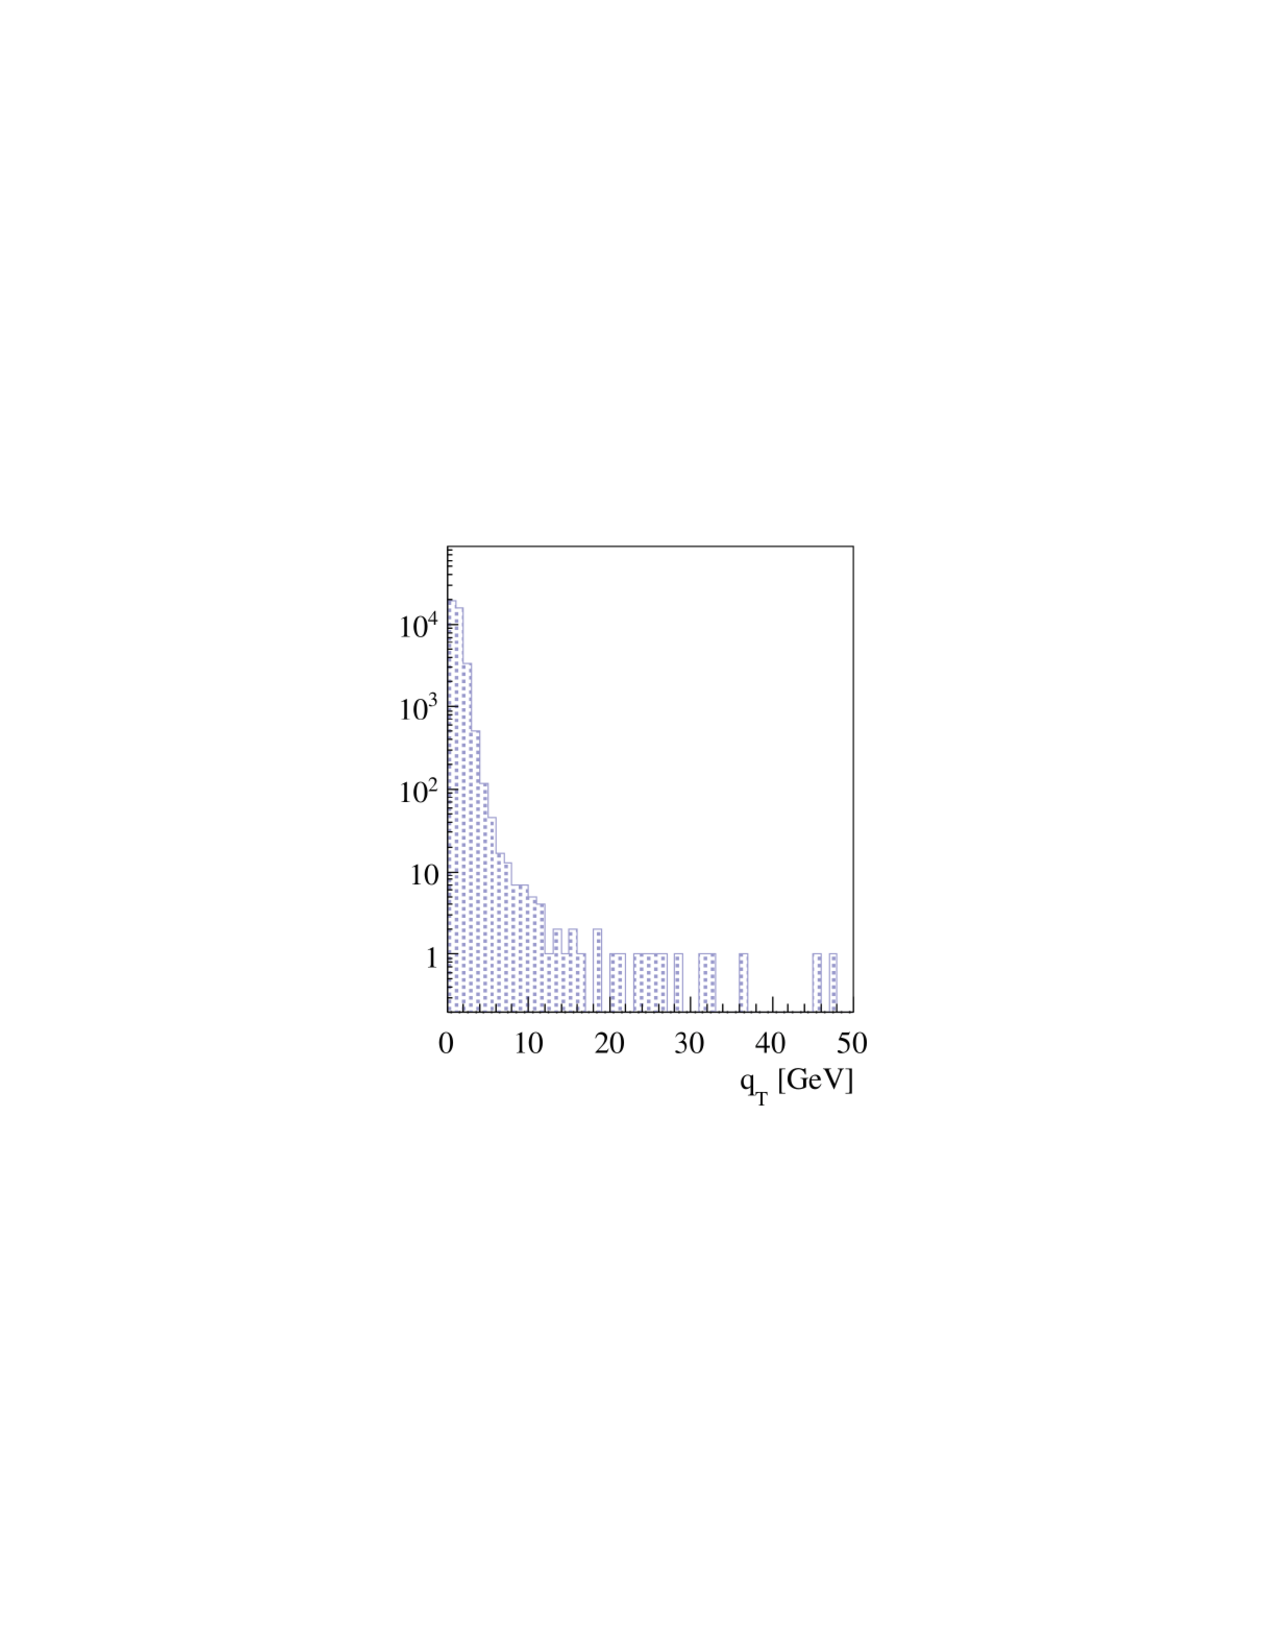
\includegraphics[width=\linewidth, trim=6cm 8.7cm 6cm 8cm,
      clip]{qT_noCuts}
    \caption{$q_T$ distribution without cuts on $q_T$.  All other cuts expect
      the $q_T$ cut from table~\ref{tab::cutdescrip} are applied.  This image is
      from~\cite{janthesis}}
    \label{fig::qT_noCuts}
  \end{subfigure}%
  \begin{subfigure}{.02\textwidth}
    \centering
    
\includegraphics[width=\linewidth]{tmp2}
    \label{fig::tmp2}%
  \end{subfigure}
  \begin{subfigure}{.46\textwidth}
    \centering 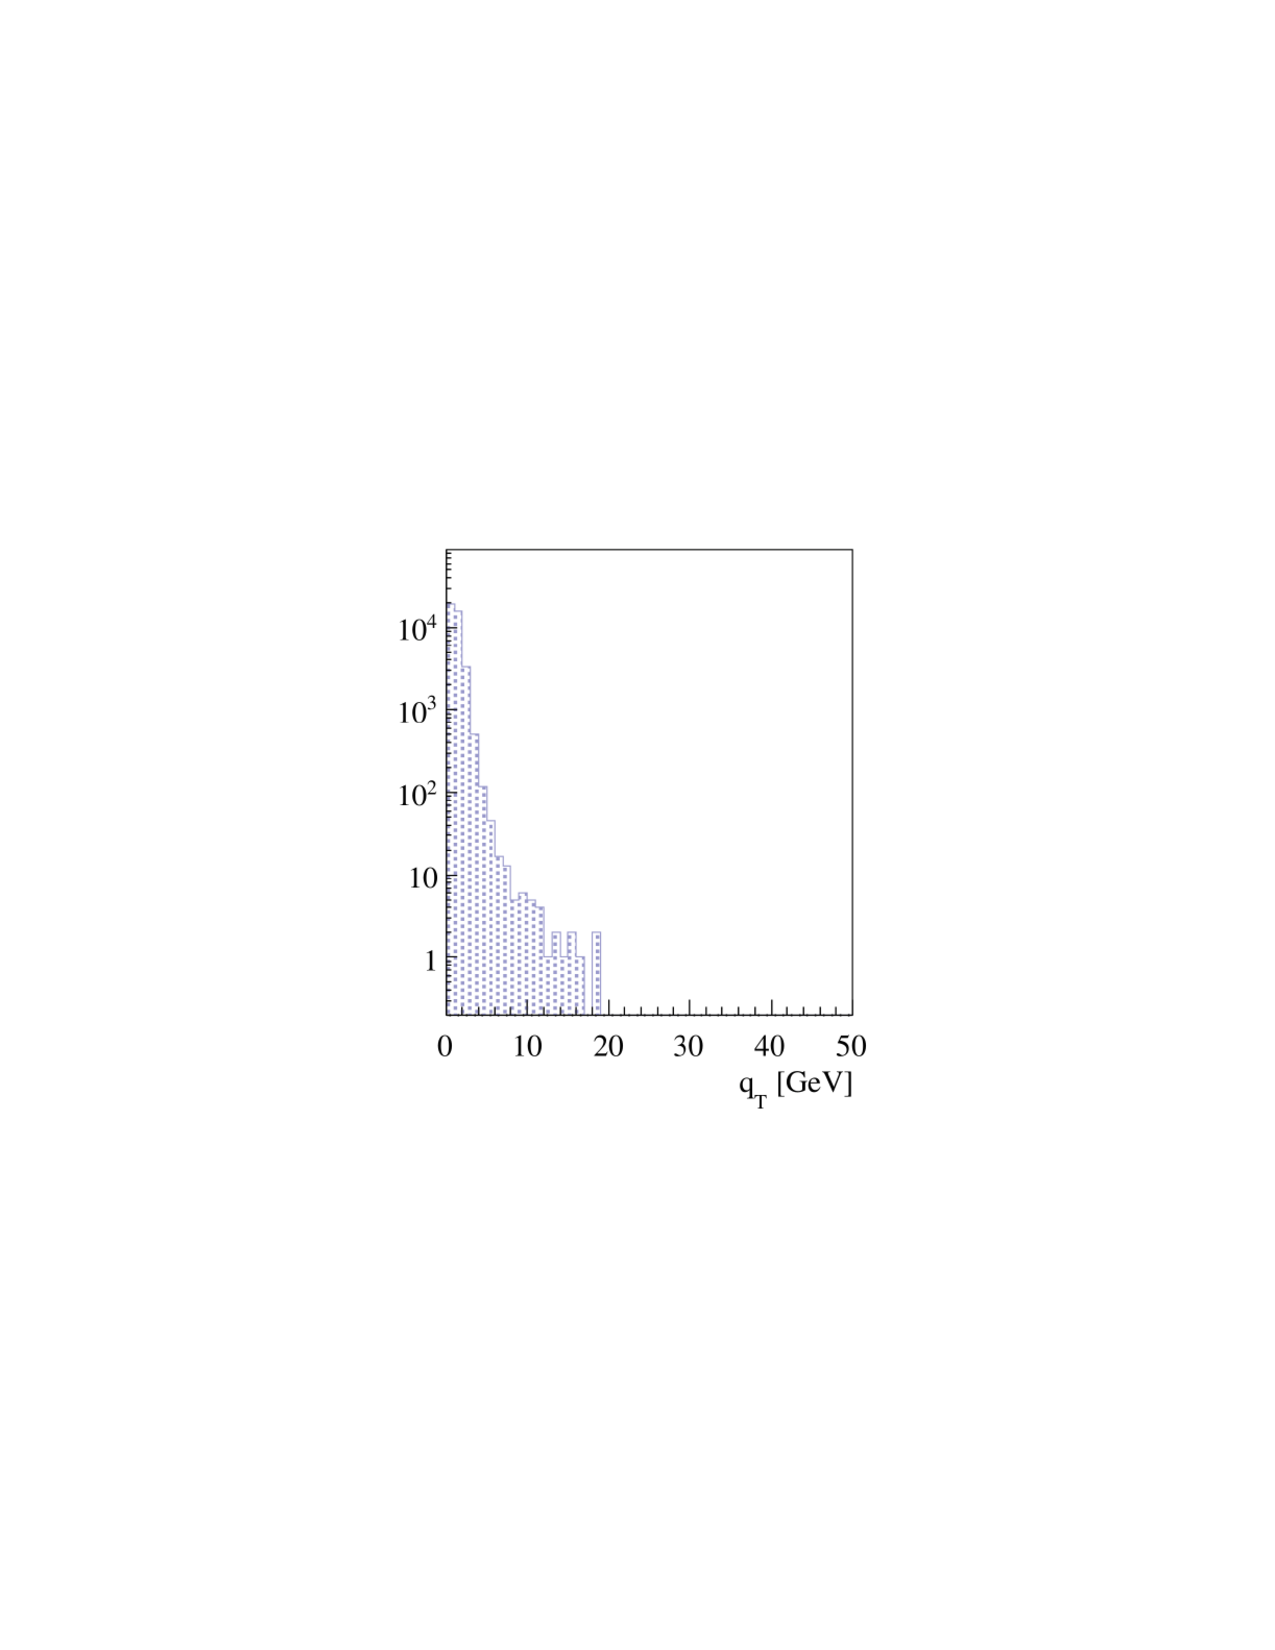
\includegraphics[width=\linewidth, trim=6cm 9cm 6cm 8cm,
      clip]{qT_PconserveCut}
    \caption{$q_T$ distribution after the momentum conservation cut is added,
      $\ell^+ \; + \; \ell^- \; < \; 190$ GeV/c.  All other cuts expect the
      $q_T$ cut from table~\ref{tab::cutdescrip} are applied.  This image is
      from~\cite{janthesis}}
    \label{fig::qT_PconserveCut}
  \end{subfigure}
\end{figure}

\begin{figure}[h!t]
  \centering
    \begin{tabular}{ |c|c|c| }
      \hline \textbf{Cuts}& \textbf{Events} & \textbf{\% Remaining} \\ \hline

      \multirow{2}{15em}{$\mu^+\mu^-$ from best primary vertex,
        4.3$<M_{\mu\mu}<8.5$ GeV/c$^2$}& 1,159,349& 100.00\\ & & \\ \hline
      
      \multirow{2}{14em}{Triggers: (2LAS or LASxOT) and not LASxMiddle}& 
      868,291& 74.89\\ & & \\ \hline
      
      Z$_{first} <$ 300 cm, Z$_{last} >$ 1500 cm& 784,379& 67.66\\ \hline

      $\Delta$t defined& 776,643& 66.99\\ \hline
      
      $|\Delta\mathrm{t}| <$ 5 ns& 337,081& 32.18\\ \hline

      $\chi^2_{track}$/ndf $<$ 10& 370,054& 31.92\\ \hline

      $\ell^+ + \ell^- < 190$ GeV/c& 219,304& 18.92\\ \hline

      $\ell_T^\pm < 7$ GeV/c& 219,014& 18.89\\ \hline

      Trigger Validation& 168,939& 14.57\\ \hline

      Good Spills& 137,812& 11.89\\ \hline

      0$<$ x$_{\pi}$ x$_N$ $<$1, -1$<$ x$_F$ $<$1& 137,802& 11.89  \\ \hline

      Z Vertex within NH$_3$& 42,646& 3.68\\ \hline

      Vertex Radius $<$ 1.9cm& 39,088& 3.37\\ \hline

    \end{tabular}
    \caption{Event selection statistics for $q_T$-weighed asymmetry analysis
      from all periods combined}
    \label{tab::qt_EventTable}
\end{figure}

\subsection{Binning}
The asymmetry is determined in bins of physical kinematic variables and an
overall integrated value.  The binning kinematical variables are $x_N$, $x_\pi$,
$x_F$ and $M_{\mu\mu}$ which are the same as the left-right asymmetry and double
ratio kinematical variables without the $q_T$ binning.  No $q_T$ binning is used
because full integrated of the $q_T$ variable needs to be taken into account to
form the weighted asymmetry.  The binning boundaries for the physical kinematics
are the same as that of the left-right asymmetry and are provided in
Tab~\ref{tab::binning}.

\subsection{Asymmetry Method}
The weighted asymmetry amplitudes $A_T^{\sin(\phi_S) q_T/M_N}$,
$A_T^{\sin(2\phi+\phi_S) q^3_T/(2M_{\pi}M_N^2)}$ and $A_T^{\sin(2\phi-\phi_S)
  q_T/M_{\pi}}$ are all determined using a modified double ratio.  As with the
double ratio method from Sec~\ref{sec::doubleratio}, the modified double ratio
does not depend on the spectrometer acceptance.  The modified double ratio is
defined as

\begin{equation}
  \label{equ::modified_dr}
  R^W_{DM}(\Phi)=
  \frac{N^{\uparrow W}_{1}N^{\uparrow W}_{2}
    - N^{\downarrow W}_{1}N^{\downarrow W}_{2}}
       {\sqrt{(N^{\uparrow W}_{1}N^{\uparrow W}_{2}
         + N^{\downarrow W}_{1}N^{\downarrow W}_{2})
         (N^{\uparrow}_{1}N^{\uparrow}_{2}
         + N^{\downarrow}_{1}N^{\downarrow}_{2})}},
\end{equation}
\noindent
where similar notation is used from the previous analyses with
$\uparrow(\downarrow)$ giving the transverse polarization direction, 1(2) is the
upstream(downstream) cell, $N^{W}$ representing the weighted counts, $W$ being
the weight used and $N$ being the unweighted counts.  The angles $\Phi$, in the
modified double ratio, are the same used for the double ratio,
Eq.~\ref{equ::ratio_phiAngles}, and give access to asymmetry amplitudes related
to the same corresponding TMD functions.  Under the same reasonable acceptance
ratio assumption, Eq.~\ref{equ::a_resonable_assump}, from the double ratio
method the acceptance cancels out in the double ratio method.  The modified
double ratio then reduces to

\begin{equation}
  \label{equ::dr_fit_form}
  R^W_{DM}(\Phi) \approx 2 \tilde{D}_{\sin\Phi}\langle S_T \rangle
  A_T^{\sin(\Phi)W} \sin\Phi,
\end{equation}
\noindent
where $\tilde{D}_{\sin\Phi}$ is an integrated depolarization factor defined as

\begin{equation}
  \tilde{D}_{\sin\phi_S} = 1, \quad\quad \tilde{D}_{\sin(2\phi\pm\phi_S)} =
  \frac{\int a(\theta)\sin^2\theta d\cos\theta} {\int a(\theta)(1+\cos^2\theta)
    d\cos\theta} = \frac{1-\langle \cos^2\theta\rangle} {1+\langle
    \cos^2\theta\rangle}.
\end{equation}

The statistical error for the modified double ratio is

\begin{equation}
  \sigma^2{R^W_{DM}} = \frac{\sum_{c,p} \sigma^2_{N_c^{pW}}
    4(N^{\uparrow}_1N^{\uparrow}_2)N^{\downarrow}_1N^{\downarrow}_2)^2}
        {\sum_{c,p} \sigma^2_{N_c^{p}}
          (N^{\uparrow}_1N^{\uparrow}_2 + N^{\downarrow}_1N^{\downarrow}_2)^4}
        \sum_{c,p}\frac{1}{N_c^p},
\end{equation}
\noindent
where $\sigma^2_{N_c^{pW}} = \sum (W^p_c)^2$ is the sum of event weights, $c$ is
cell 1 or cell 2 and $p$ is polarization $\uparrow$ or $\downarrow$.

The weighted asymmetry amplitude are determined by forming the modified double
ratio in eight bins in the appropriate $\Phi$ angle and fitting this
distribution.  If an infinite number of bins where used, the modified double
ratio distribution would be the function form of Eq.~\ref{equ::dr_fit_form}.  To
account for the fact that ratio is determined in a finite number of $\Phi$ bins,
the average value of Eq.~\ref{equ::dr_fit_form} over the bin width is used as
the fit distribution.  This means the functional fit is

\begin{equation}
  \langle R^W_{DM} \rangle = \frac{1}{\Delta\Phi}
  \int_{\Phi_i-\frac{\Delta\Phi}{2}}^{\Phi_i+\frac{\Delta\Phi}{2}} R^W_{DM}
  d\Phi = \frac{2}{\Delta\Phi}\sin(\frac{\Delta\Phi}{2})R^W_{DM}(\Phi_i),
\end{equation}
\noindent
where $\Delta\Phi$ = $\frac{2\pi}{8}$ for eight bins in $\Phi$.

\subsection{Results}
As with the other analyses in this thesis, the asymmetry amplitudes are
determine for each period and the final asymmetry is determined as a period
weighted average as in Eq.~\ref{equ::wAvg}.  For the same reason as the previous
analyses and explained in Sec~\ref{sec::lr_results}, the polarization and
depolarization factors from each period are used to correct the asymmetry
amplitude determined in each period.  The final results are shown in
Fig.~\ref{fig::wA_results} along with the results from the release values.  As
can be seen the results agree with those results obtained for the release which
was a requirement before the result could be release to the public.

\begin{figure}[h!t]
  \centering 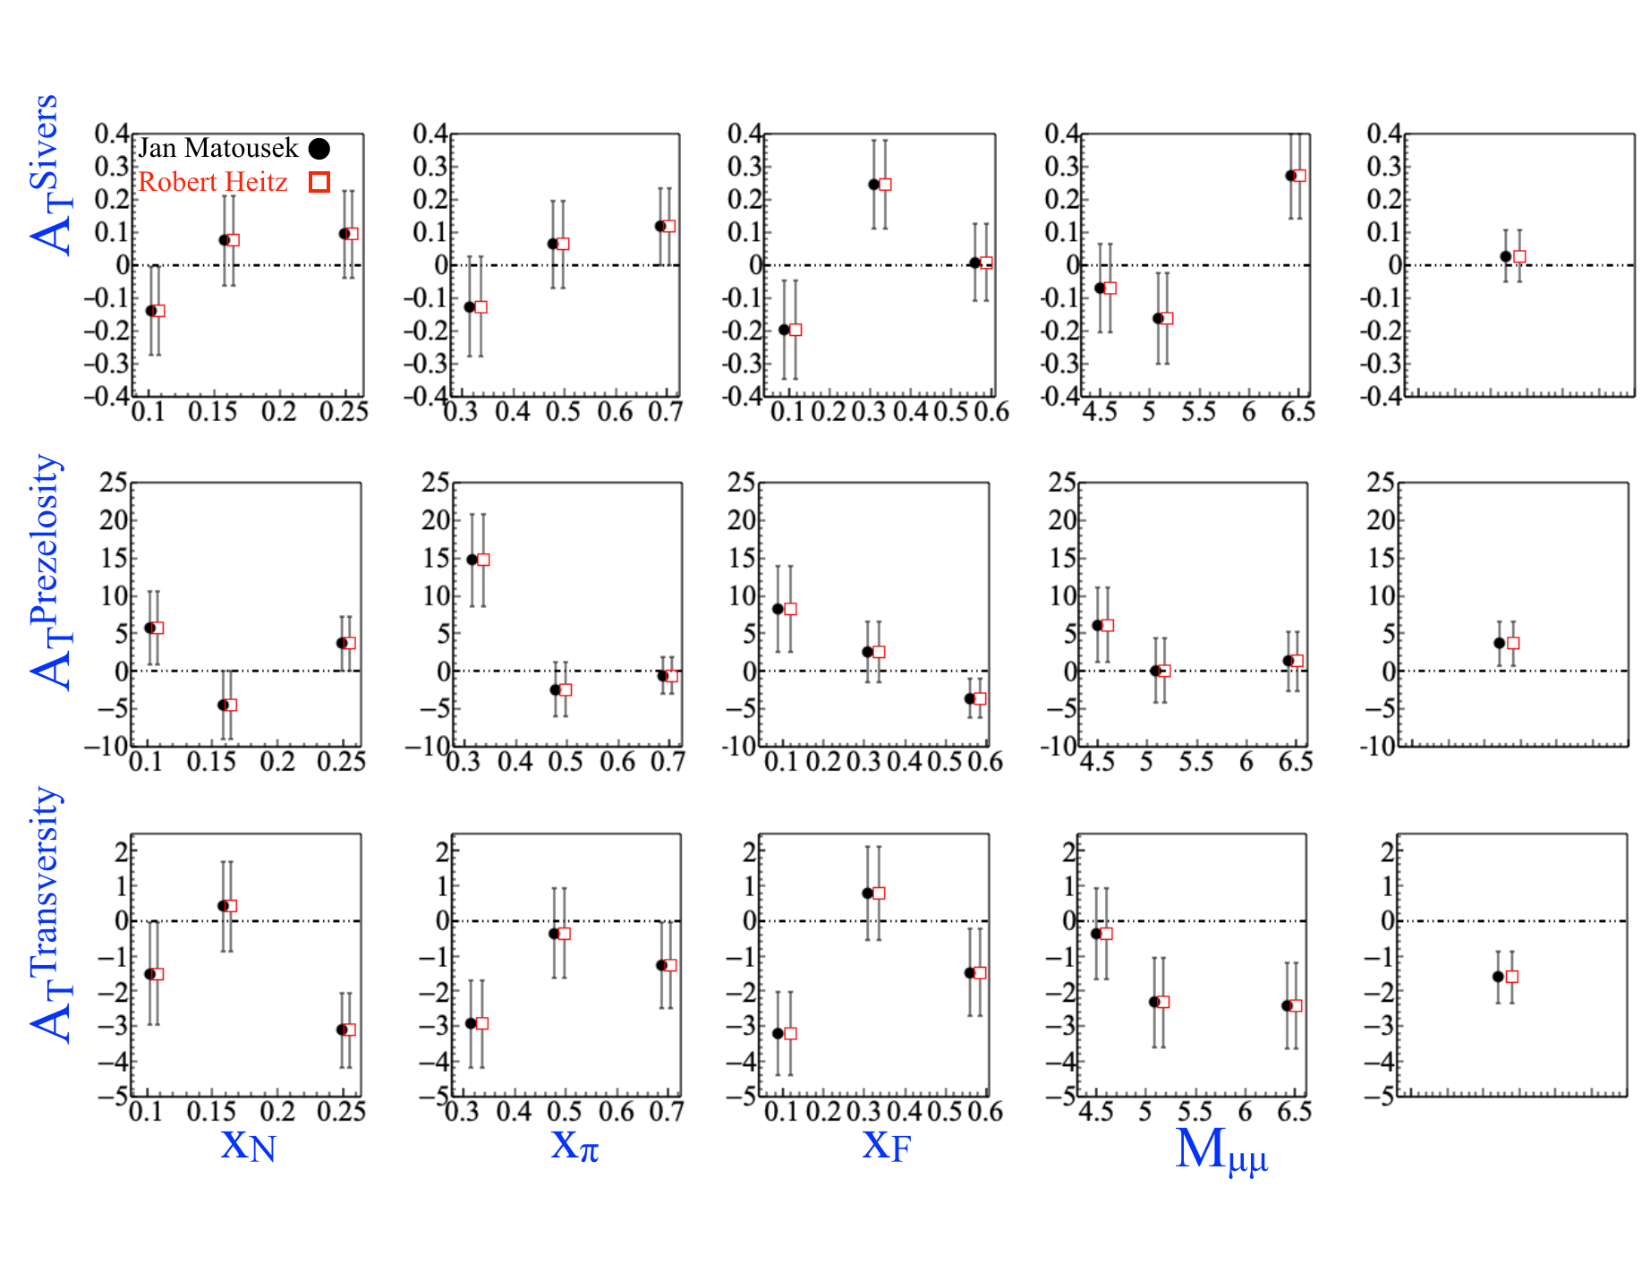
\includegraphics[width=\textwidth,trim=0.2cm 1.5cm 0.2cm 1.5cm,
    clip]{wA_results}
  \caption{The comparison of weighted asymmetry amplitude results from the
    released values from Jan Matousek (black) and the cross checker Robert Heitz
    (red).  From the top row down the asymmetry amplitudes are
    $A_T^{\sin(\phi_S) q_T/M_N}$, $A_T^{\sin(2\phi+\phi_S)
      q^3_T/(2M_{\pi}M_N^2)}$ and $A_T^{\sin(2\phi-\phi_S) q_T/M_{\pi}}$
    respectively.}
  \label{fig::wA_results}
\end{figure}


